\documentclass[10pt, twoside, openany]{book}

\usepackage[a4paper, top=2.5cm, bottom=2.5cm, left=3cm, right=3cm]{geometry}
\usepackage[utf8]{inputenc}
\usepackage[italian]{babel}
\usepackage{cite}
\usepackage[numbers, sort&compress]{natbib}
\usepackage{hyperref}
\usepackage{graphicx}
\usepackage{fancyhdr}
\usepackage[Lenny]{fncychap}
\usepackage{frontespizio}
\usepackage{tabularx}
\usepackage{caption}
\usepackage{amsmath}

\pagestyle{fancy}
\fancyhead{}
\fancyhead[LE]{\nouppercase{\leftmark}}
\fancyhead[RO]{\nouppercase{\rightmark}}
\bibliographystyle{unsrtnat} %Ordine dei riferimenti bibliografici = ordine con cui le citazioni compaiono nel testo.

\begin{document}
\begin{frontespizio}
\Universita{Roma Tor Vergata}
\Dipartimento{Ingegneria Civile e Ingegneria dell'Informazione}
\Corso{Ingegneria Informatica}
\Annoaccademico{2023/2024}
\Titolo{Titolo della tesi}
\Candidato[0316179]{Matteo Fanfarillo}
\Relatore{Giuseppe Bianchi}
\Correlatore{Francesco Gringoli}
\Logo{logo.png}
\end{frontespizio}

\begin{flushright}
\null\vspace{\stretch{1}}
\textit{[Citazione]}
\vspace{\stretch{2}}\null
\end{flushright}

\tableofcontents
\listoffigures
\listoftables

\chapter{Introduzione}
\section{Panoramica sull'eSIM}
La eSIM (embedded-SIM) non è altro che una SIM virtuale: grazie a lei, quando l'utente vuole cambiare operatore, non deve più acquistare fisicamente una nuova SIM card presso un negozio del nuovo operatore, bensì gli è sufficiente ricevere via e-mail un profilo, ossia una "SIM digitale" che può essere caricata subito sul telefono mediante la scansione di un QR code. Si tratta di una soluzione molto più pratica rispetto a recarsi fisicamente presso il negozio dell'operatore, tant'è vero che negli ultimi anni si sta diffondendo sempre di più: uno studio di Juniper Research stima che il numero di telefoni che utilizzano la connettività eSIM aumenterà dai 986 milioni attuali ai 3.5 miliardi entro il 2027 \cite{Corcom}. Per questi motivi, e poiché le informazioni associate alla comunicazione tra eSIM sono sensibili, è fondamentale garantire un livello di sicurezza sufficientemente elevato per il funzionamento dell'eSIM sia a run-time che a boot-time.

\section{Obiettivo del lavoro}
La presente trattazione si propone di effettuare un'analisi di sicurezza e delle vulnerabilità della eSIM e del suo funzionamento e, successivamente, di tentare di sfruttare, anche con delle attività di laboratorio, le eventuali vulnerabilità trovate.

\section{Definizioni preliminari}
\begin{itemize}
\item \textbf{eUICC (embedded Universal Integrated Circuit Card)}: è un chip utilizzato all'interno dei telefoni all'interno del quale è embeddato il software dell'eSIM. È integrato direttamente nei dispositivi (i.e. non è rimovibile) ed è progettato per essere programmato a distanza. Può contenere uno o più profili eSIM.
\item \textbf{LPA (Local Profile Assistant)}: è un'applicazione che vive nel telefono dell'utente ed è responsabile della gestione dei profili all'interno della rete mobile, inclusi la creazione, l'aggiornamento e la cancellazione.
\item \textbf{SM-DP+ (Subscription Manager Data Preparation plus)}: è un protocollo che rappresenta una tecnica di provisioning usata per configurare le eSIM in modo automatico e remoto. Rispetto alla versione base SM-DP, offre delle funzionalità aggiuntive come un sistema di crittografia più avanzato e un'architettura di rete più flessibile.
\end{itemize}

\section{Panoramica sui capitoli successivi}
Nel capitolo 2 verrà svolta una trattazione dettagliata sull'architettura e sulle interfacce dell'eSIM, con lo scopo di fornire al lettore gli strumenti per comprendere appieno le tematiche centrali del lavoro. Nel capitolo 3 verrà effettuata un'analisi della sicurezza dell'eSIM a run-time, mentre nel capitolo 4 si procederà con l'analisi della sicurezza dell'eSIM a boot-time (i.e. durante la fase di configurazione). Infine, nel capitolo 5 verranno mostrati i risultati finali, verranno tratte delle conclusioni sul lavoro svolto e verrà fornita una panoramica sui possibili progetti futuri che potranno essere intrapresi a partire dai risultati ottenuti attraverso questo lavoro.

\chapter{Interfacce e funzionamento dell'eSIM}
\section{Architettura di RSP}
Per comprendere appieno come funziona e come si interfaccia l'eSIM all'interno dei dispositivi mobili, è necessario introdurre il protocollo RSP, anche perché la eSIM si colloca proprio all'interno dell'architettura di RSP.\\
RSP (Remote SIM Provisioning) è un protocollo utilizzato dal protocollo SM-DP+ per gestire la comunicazione tra il server SM-DP+ e la scheda eSIM del dispositivo mobile (i.e. l'eUICC). In particolare, definisce le operazioni di provisioning specifiche per la comunicazione dell'eUICC. Quest'ultimo comprende i dati sia dell'operatore che dell'utente che, nel caso delle SIM tradizionali, verrebbero appunto memorizzati su una SIM card fisica. Entrando più nel dettaglio sul funzionamento di RSP, l'end user che vuole ottenere un profilo eSIM offerto da un particolare operatore (nel quale viene definito un piano tariffario), deve pagare l'operatore affinché esso gli fornisca un codice QR. Dopodiché, deve effettuare la scansione di tale codice QR per avviare lo scaricamento (operazione di Download) e l'installazione (operazione di Install) del profilo eSIM: a questo punto, la connessione tra end user (col relativo profilo eSIM) e operatore è completata. Se in un secondo momento l'end user ha la necessità di ottenere e utilizzare un secondo profilo eSIM, gli è sufficiente ripetere i medesimi passaggi appena descritto, e questo secondo profilo può essere installato all'interno del medesimo eUICC che ospita già il primo profilo. Tale meccanismo è illustrato nella figura \ref{fig:RSP-functioning} tratta da \cite{GSMA-whitepaper}.
\begin{figure}
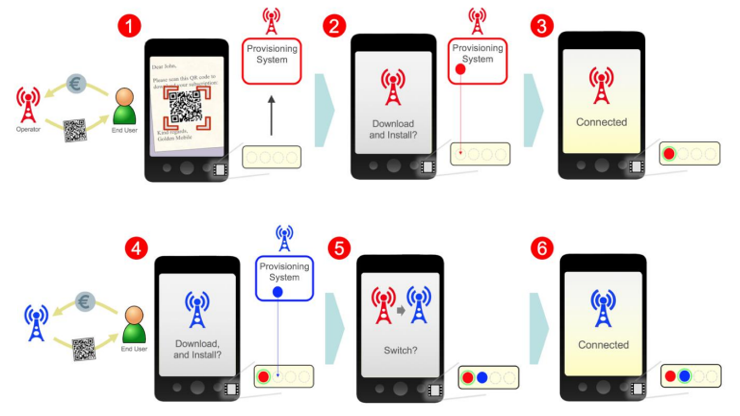
\includegraphics[width=\linewidth]{RSP-functioning.png}
\caption{Comunicazione tra end user e operatore nel contesto del Remote SIM Provisioning.}
\label{fig:RSP-functioning}
\end{figure}
\\Per quanto riguarda l'architettura interna di RSP nello specifico, esistono due soluzioni differenti \cite{GSMA-docs}.
\begin{enumerate}
\item \textbf{LPA embeddato nel dispositivo mobile ma non all'interno dell'eUICC (LPAd)}: oltre alla comunicazione tra l'applicazione LPA e SM-DP+, si utilizzano delle apposite interfacce anche per la comunicazione tra l'eUICC e l'applicazione LPA, come mostrato nella figura \ref{fig:RSP-LPAd} tratta da \cite{GSMA-docs}.
\begin{figure}
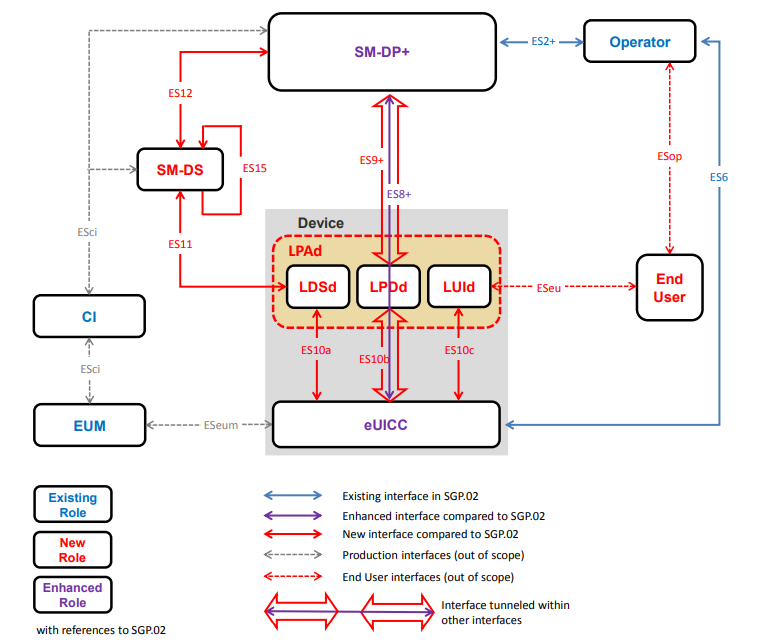
\includegraphics[width=\linewidth]{RSP-LPAd.png}
\caption{Architettura di RSP nel caso di LPA non embeddato nell'eUICC.}
\label{fig:RSP-LPAd}
\end{figure}
Di seguito è riportato un breve glossario che chiarisce il significato di alcuni componenti appartenenti all'architettura di RSP raffigurata in \ref{fig:RSP-LPAd}.
\begin{itemize}
\item \textbf{CI} = Certificate Issuer: è un'entità autorizzata a rilasciare certificati digitali.
\item \textbf{EUM} = eUICC Manufacturer: è il fornitore delle eUICC e del software residente (e.g. firmware, sistema operativo); svolge anche il ruolo di certificate authority subordinata al CI e rilascia certificati all'eUICC \cite{Sec-analysis}.
\item \textbf{LDSd} = Local Discovery Service (quando LPA non è nell'eUICC).
\item \textbf{LPDd} = Local Profile Download (quando LPA non è nell'eUICC).
\item \textbf{LUId} = Local User Interface (quando LPA non è nell'eUICC).
\item \textbf{SM-DS} = Subscription Manager Discovery Server: è il componente che fornisce un mezzo a SM-DP+ per raggiungere l'eUICC senza dover sapere a quale rete il dispositivo è connesso.
\end{itemize}
\item \textbf{LPA embeddato all'interno dell'eUICC (LPAe)}: sono necessarie solo delle interfacce tra l'eUICC e SM-DP+, come mostrato nella figura \ref{fig:RSP-LPAe} tratta da \cite{GSMA-docs}.
\begin{figure}
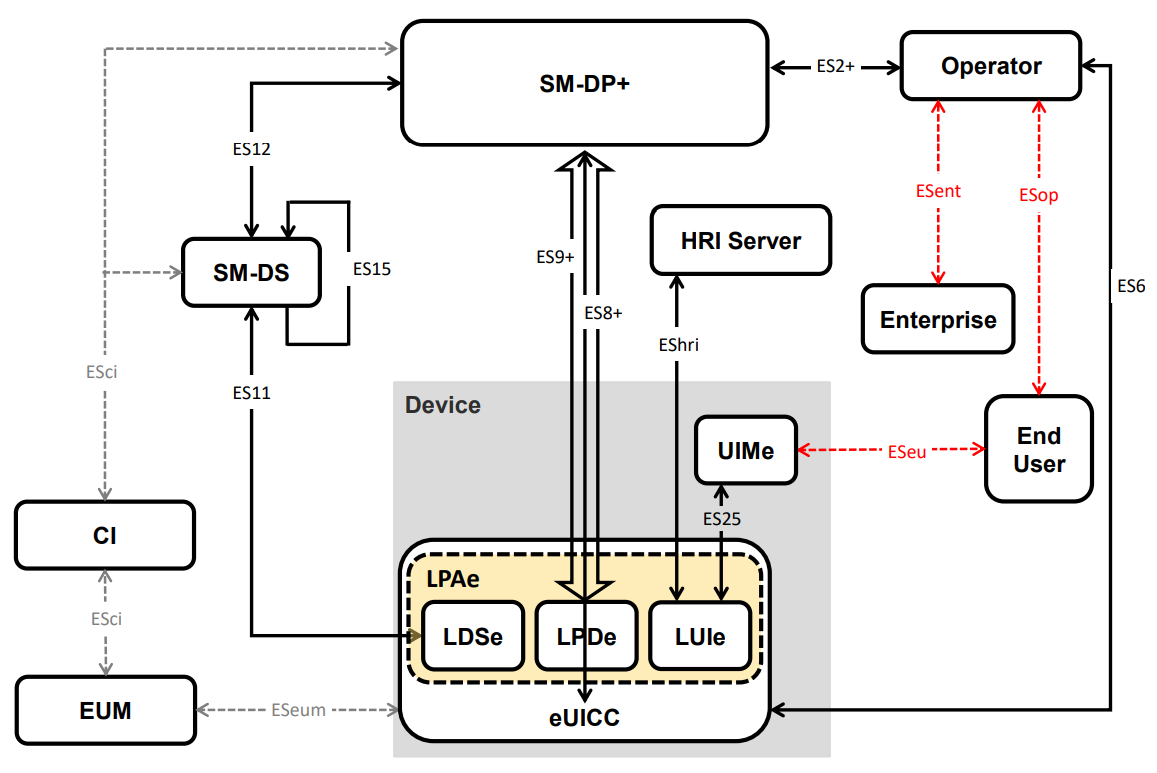
\includegraphics[width=\linewidth]{RSP-LPAe.png}
\caption{Architettura di RSP nel caso di LPA embeddato nell'eUICC.}
\label{fig:RSP-LPAe}
\end{figure}
Successivamente è riportato un breve glossario che chiarisce il significato di alcuni componenti appartenenti all'architettura di RSP raffigurata in \ref{fig:RSP-LPAe}.
\begin{itemize}
\item \textbf{LDSe} = Local Discovery Service (quando LPA è nell'eUICC).
\item \textbf{LPDe} = Local Profile Download (quando LPA è nell'eUICC).
\item \textbf{LUIe} = Local User Interface (quando LPA è nell'eUICC).
\end{itemize}
\end{enumerate}

\subsection{Interfacce presenti nell'architettura di RSP}
Sono illustrate nella tabella \ref{tab:interfaces}, costruita a partire da informazioni tratte da \cite{GSMA-docs}.
\begin{table}[h!]
\begin{center}
\captionsetup{skip=4pt}
\caption{Interfacce in RSP}
\label{tab:interfaces}
\begin{tabularx}{\textwidth}{|c|c|c|X|} % <-- Alignments: 1st column center, 2nd center and 3rd center, with vertical lines in between
\hline
\textbf{Interfaccia} & \textbf{Componente 1} & \textbf{Componente 2} & \textbf{Descrizione}\\
\hline
ES2+ & Operatore & SM-DP+ & Viene usata dall'operatore per invocare la preparazione del Profile Package*.\\
\hline
ES6 & Operatore & eUICC & Viene usata dall'operatore per gestire il contenuto dei profili.\\
\hline
ES8+ & SM-DP+ & eUICC & Fornisce un canale end-to-end sicuro tra SM-DP+ e l'eUICC per l'amministrazione dell'ISD-P** e del relativo profilo durante il download e l'installazione.\\
\hline
ES9+ & SM-DP+ & LPD & Viene usata per fornire trasporto sicuro tra SM-DP+ e LPD per la consegna del Profile Package.\\
\hline
ES10a & LDSd & eUICC & Viene usata da LPAd per ottenere gli indirizzi configurati dall'eUICC per Root SM-DS*** (gestione di una Discovery Request).\\
\hline
ES10b & LPDd & eUICC & Viene usata da LPAd per trasferire un Profile Package all'eUICC.\\
\hline
ES10c & LUId & eUICC & Viene usata da LPAd per la gestione locale dei profili installati sull'eUICC da parte dell'end user (e.g. Enable, Disable, Delete).\\
\hline
ES11 & LDS & SM-DS & Viene usata per l'ottenimento di eventi.\\
\hline
ES12 & SM-DP+ & SM-DS & Viene usata per la gestione degli eventi.\\
\hline
ES15 & SM-DS & SM-DS & Viene usata per connettere gli SM-DS tra loro nel caso in cui ce ne sia più di uno.\\
\hline
ESop & Operatore & End user & È specifica per le relazioni di business tra l'operatore e l'end user.\\
\hline
ESeu & End user & LUI & È specifica per le relazioni di business tra l'end user e la LUI.\\
\hline
ESeum & eUICC & EUM & È specifica per le relazioni di business tra l'eUICC e l'EUM.\\
\hline
ESci & CI & SM-DP+, SM-DS, EUM & Viene usata per richiedere certificati.\\
\hline
\end{tabularx}
\end{center}
\end{table}
\\**Un Profile Package è un pacchetto di dati associato a un profilo che contiene le informazioni di configurazione necessarie per attivare e utilizzare quel profilo all'interno di una scheda eSIM. Esistono diversi tipi di Profile Package: l'Unprotected Profile Package (UPP) è un pacchetto di dati non protetto da alcun meccanismo di sicurezza, come l'autenticazione o la crittografia; il Protected Profile Package (PPP) è un pacchetto di dati protetto da alcuni meccanismi di sicurezza; il Bound Profile Package (BPP) è un pacchetto di dati legato a un particolare dispositivo o a una piattaforma di servizi; il Segmented Bound Profile Package (SBPP), infine, non è altro che un BPP suddiviso in molteplici segmenti che possono essere utilizzati in modo indipendente e separato.\\
***ISD-P (Issuer Security Domain Profile) è un contenitore sicuro che ospita un unico profilo.\\
****Root SM-DS è il server primario utilizzato da un operatore di rete mobile per gestire le attivazioni e le disattivazioni delle sottoscrizioni e per gestire funzionalità come l'autenticazione e l'autorizzazione degli utenti. D'altra parte, si hanno gli Alternative SM-DS, che sono server di backup a cui si ricorre quando il Root SM-DS non è disponibile.

\section{Architettura dell'eUICC}
Nella figura \ref{fig:eUICC-arch} tratta da \cite{GSMA-docs} è schematizzata l'architettura interna del chip eUICC, dove i riquadri e le frecce in rosso sono relativi rispettivamente ai componenti e alle interfacce che, nell'ambito dell'eUICC, sono presenti esclusivamente nel caso in cui l'applicazione LPA sia effettivamente embeddata all'interno dell'eUICC (LPAe).
\begin{figure}
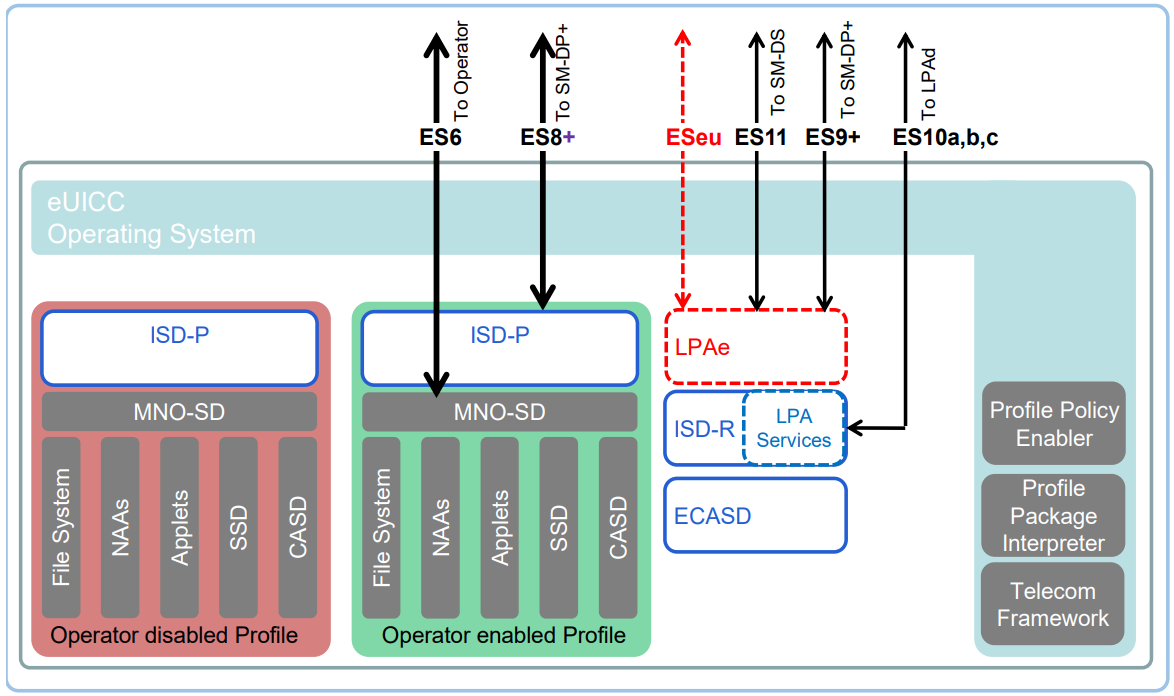
\includegraphics[width=\linewidth]{eUICC-arch.png}
\caption{Architettura dell'eUICC.}
\label{fig:eUICC-arch}
\end{figure}
\\Di seguito, invece, è riportato un breve glossario che chiarisce il significato di alcuni componenti appartenenti all'architettura dell'eUICC raffigurata in \ref{fig:eUICC-arch}.
\begin{itemize}
\item \textbf{CASD} = Controller Authority Security Domain: è un'area di storage sicura all'interno dell'ISD-P in cui vengono memorizzate le credenziali richieste per supportare le funzionalità di sicurezza sensibili.
\item \textbf{ECASD} = Embedded Controller Authority Security Domain: è il componente CASD direttamente incapsulato all'interno dell'eUICC.
\item \textbf{ISD-R} = Issuer Security Domain Root: è il componente responsabile della creazione di nuovi ISD-P e della gestione del loro ciclo di vita.
\item \textbf{LPA Services} = i seguenti quattro servizi: trasferimento del Bound Profile Package da LPAd all'ISD-P; ottenimento della lista dei profili installati; recupero dell'EID (eUICC ID); ottenimento delle operazioni di gestione del profilo locale (Local Profile Management Operations).
\item \textbf{MNO-SD} = Mobile Network Operator Security Domain: è la parte del profilo posseduta dall'operatore che fornisce all'operatore Over The Air (OTA) un canale di comunicazione sicuro; viene usato per gestire il contenuto di un profilo una volta che è stato abilitato.
\item \textbf{NAAs} = Network Access Applications: sono le applicazioni che consentono l'accesso alla rete.
\item \textbf{Profile Package Interpreter} = servizio del sistema operativo dell'eUICC che traduce i dati del Profile Package in un profilo installato all'interno dell'ISD-P codificando usando il formato interno dell'eUICC.
\item \textbf{Profile Policy Enabler} = componente che verifica che un il profilo eSIM possa essere installato sull’eUICC.
\item \textbf{SSD} = Supplementary Security Domain: è un'area di memoria protetta all'interno dell'ISD-P che viene utilizzata per l'esecuzione di funzioni di sicurezza come le operazioni crittografiche. Di fatto, il suo scopo principale è quello di proteggere le informazioni riservate dell'utente (i.e. chiavi, password) da accessi non autorizzati e attacchi esterni.
\item \textbf{Telecom Framework} = servizio del sistema operativo dell'eUICC che fornisce algoritmi di autenticazione di rete standardizzati alle applicazioni NAAs ospitate nei rispettivi ISD-P.
\end{itemize}

\subsection{Caratteristiche hardware e software dell'eUICC}
\begin{enumerate}
\item Deve essere resistente al tampering dei componenti hardware.
\item Supporta SHA-1.
\item Supporta TUAK, che è un particolare algoritmo crittografico di 3GPP, dove 3GPP (Third Generation Partnership Project) è il consorzio industriale che definisce gli standard per la tecnologia 5G .
\item Supporta Milenage, che è un set di funzioni 3GPP di autenticazione e di key generation.
\item Tutte le funzioni crittografiche devono essere resistenti al tampering e agli attacchi side-channel.
\end{enumerate}

\section{Interazione tra eUICC, LPA, SM-DP+ e operatore}
\subsection{Sicurezza TLS}
Il protocollo TLS, la cui versione 1.2 è definita in RFC 5246 \cite{RFC-5246} e la cui versione 1.3 è definita in RFC 8446 \cite{RFC-8446}, è utilizzato per proteggere il traffico sulle interfacce ES2+ (tra server SM-DP+ e operatore) e ES9+ (tra server SM-DP+ e LPA). In particolare, in ES2+ è prevista la mutua autenticazione tra le parti, mentre in ES9+ è prevista solo l'autenticazione del server. La documentazione di GSMA di riferimento \cite{GSMA-docs} sottolinea l'obbligatorietà di fare uso di TLS v1.2 sia per gli algoritmi di autenticazione e autorizzazione, sia per l'integrità dei messaggi, sia per la confidenzialità. In realtà, documenti più recenti di GSMA \cite{GSMA-docs2} introducono la possibilità (e suggeriscono) di utilizzare TLS v1.3, che è la versione più recente di TLS e risolve le vulnerabilità che caratterizzano TLS v1.2, per cui, in linea di principio, dovrebbe risultare particolarmente difficoltoso da penetrare. Tuttavia, attualmente sembra essere solo un suggerimento, per cui nei capitoli successivi potrebbe essere necessario verificare a livello pratico qual è la versione di TLS utilizzata per proteggere la comunicazione tra LPA e server SM-DP+.\\
Un discorso analogo vale per l'interazione che si ha nella mutua autenticazione tra l'eUICC e il server SM-DP+, dove le due parti interagiscono tra loro tramite un TLS tunnel \cite{Sec-analysis}. Per quanto invece riguarda la comunicazione tra eUICC e applicazione LPA, è richiesto l'utilizzo di un pairwise secure channel (ovvero di un canale di comunicazione sicuro rispetto alla confidenzialità e all'autenticazione dei messaggi) che collega le due parti all'interno del dispositivo mobile \cite{Sec-analysis}. Tuttavia, non esiste una specifica universale che imponga l'utilizzo di un particolare protocollo di crittografia per proteggere il pairwise secure channel; il protocollo più utilizzato a tal proposito rimane TLS ma, di nuovo, potrebbe essere necessario stabilire con un approccio pratico se nel canale di comunicazione tra eUICC e LPA viene utilizzato TLS oppure un protocollo differente.

\subsection{Dettagli sull'interazione in RSP}\label{sec:RSP-interaction}
L'interazione tra le parti, nel contesto del protocollo RSP, avviene in quattro fasi distinte: profile ordering, download initialization, common handshake e profile download \cite{Sec-analysis}.
\begin{itemize}
\item \textbf{Profile ordering \& download initialization}: nella prima fase, l'operatore richiede al server SM-DP+ di preparare un profilo eSIM, e il server gli restituisce dei download initialization pointer (che possono essere rappresentati ad esempio da un codice di attivazione). Nella seconda fase, invece, l'operatore consegna i download initialization pointer all'LPA in modo tale che poi sia possibile effettuare il download vero e proprio del profilo. Per questi primi due step, si possono seguire tre tipi di approcci differenti:
\begin{enumerate}
\item \underline{Default server approach}: la figura \ref{fig:default-server} tratta da \cite{Sec-analysis} mostra questo approccio. L'operatore (indicato con MNO - Mobile Network Operator) pre-condivide con l'eUICC l'indirizzo S del server. Quando vuole effettuare una nuova sottoscrizione e ottenere così un nuovo profilo, l'end user contatta l'operatore (messaggio 0), il quale ordina al server SM-DP+ il profilo per l'identificatore U dell'eUICC target (messaggio 1). Il server crea il nuovo profilo e lo invia all'operatore (messaggio 2), il quale notifica l'utente (messaggio 3). A tal punto, l'applicazione LPA viene avviata e, tramite un'operazione di get, recupera S dall'eUICC.
\item \underline{Activation code approach}: la figura \ref{fig:activation-code} tratta da \cite{Sec-analysis} mostra questo secondo approccio. L'operatore ordina al server SM-DP+ dei profili (messaggio 1), e il server li rende disponibili con un codice di attivazione (tipicamente un codice QR) e li restituisce all'operatore (messaggio 2). Il codice di attivazione include l'indirizzo S del server, l'identificatore $I_{ac}$ del profilo e, opzionalmente, l'OID, ovvero l'identificatore del server SM-DP+. Quando l'end user vuole effettuare una nuova sottoscrizione e ottenere così un nuovo profilo, contatta l'operatore (messaggio 0, che può essere inviato sia prima che dopo l'interazione tra operatore e SM-DP+ server appena descritta), il quale restituisce il codice di attivazione opportuno (messaggio 3).
\item \underline{SM-DS assisted approach}: è un approccio analogo all'activation code, con la differenza che SM-DP+ si appoggia sui server SM-DS per comunicare con l'eUICC.
\end{enumerate}
\item \textbf{Common handshake}: la figura \ref{fig:common-handshake} tratta da \cite{Sec-analysis} mostra i dettagli di questa fase, che coinvolge tre attori fondamentali: il server SM-DP+, l'applicazione LPA e l'eUICC. Lo stato iniziale delle tre entità è descritto qui di seguito.
\begin{itemize}
\item Il server SM-DP+ è dotato di tre certificati, tutti e tre rilasciati dal CI: $Cert_{St}$ è il certificato TLS, $Cert_{Sa}$ è il certificato usato per autenticarsi all'eUICC e $Cert_{Sp}$ è il certificato che permette di rilasciare i profili eSIM. Il server possiede anche il profilo P che l'utente deve scaricare e il relativo identificatore \textit{mnoId} dell'operatore. Infine, ha l'identificatore U dell'eUICC target, l'identificatore $I_{ac}$ del profilo oppure entrambi.
\item L'applicazione LPA conosce l'indirizzo S del server e, opzionalmente, l'identificatore $I_{ac}$ del profilo e l'identificatore OID del server.
\item L'eUICC ha una catena di certificati composta da $Cert_{U}$ e $Cert_{EUM}$.
\end{itemize}
L'obiettivo per il server SM-DP+ e l'eUICC è quello di autenticarsi vicendevolmente all'interno di un tunnel TLS. Per iniziare questo processo, l'end user chiede all'eUICC di generare un nonce $N_{U}$ (messaggio 1) e l'eUICC replica con $N_{U}$ e la chiave $SKI_{CI}$ che determina la curva ellittica che verrà usata per i certificati, le firme e l'ECDH (elliptic-curve Diffie-Hellman) key exchange (messaggio 2). L'applicazione LPA inoltra queste due informazioni al server insieme a S (messaggio 3). Il server genera così un identificatore di sessione $I_{t}$ fresh e risponde all'LPA con un messaggio firmato con la propria chiave privata $SK_{Sa}$ che comprende $I_{t}$, il nonce $N_{U}$, un altro nonce $N_{S}$ e il proprio indirizzo S (messaggio 4). L'LPA verifica l'autenticità delle informazioni contenute nel digest, ad esempio controllando il valore di S, e in caso di successo inoltra il messaggio all'eUICC con l'identificatore $I_{ac}$ del profilo (messaggio 5). Anche l'eUICC invia il proprio digest firmato con la propria chiave privata $SK_{U}$ che contiene $I_{t}$, il nonce $N_{S}$, l'indirizzo S del server e $I_{ac}$ (messaggio 6), e l'LPA inoltra tale messaggio al server (messaggio 7); è importante notare che $I_{ac}$ è non nullo solo nell'approccio activation code. Dopodiché, il server seleziona il profilo per l'eUICC in base a $I_{ac}$ (caso activation code) oppure in base all'identificatore U dell'eUICC presente in $Cert_{U}$ (caso default server). A questo punto, invia la signature di $I_{t}$ firmata con $SK_{Sp}$ (messaggio 8) e l'LPA, quando la riceve, la inoltra a sua volta all'eUICC (messaggio 9). Quest'ultimo, infine, verifica che la signature sia autentica e che i certificati $Cert_{Sa}$ e $Cert_{Sp}$ facciano riferimento allo stesso identificatore OID del server, in modo da assicurarsi che il server stesso sia effettivamente quello autorizzato.
\item \textbf{Profile download}: la figura \ref{fig:profile-download} tratta da \cite{Sec-analysis} mostra i dettagli di quest'ultima fase, che non è altro che una continuazione della common handshake. I messaggi 10, 11, 12, 13 si occupano di portare a termine un key exchange basato su elliptic-curve key agreement (ECKA), tramite il quale viene calcolato uno shared secret da cui, mediante una key derivation function (KDF), saranno derivate le chiavi di sessione k (per la cifratura) e k' (per l'integrità dei dati). Contestualmente all'authenticated key exchange, avviene il download del profilo eSIM, in cui il server SM-DP+ invia all'LPA il profilo cifrato con la chiave k e l'identificatore \textit{mnoId} dell'operatore (messaggio 12), dove entrambe le informazioni sono firmate singolarmente con la chiave k' mediante il meccanismo di message authentication code (MAC). Dopodiché, l'LPA mostra l'identificatore \textit{mnoId} all'utente, che dovrà stabilire se fa riferimento all'operatore giusto: se sì, l'LPA inoltra tutte le informazioni all'eUICC (messaggio 13) il quale, dopo aver derivato le chiavi di sessione k, k', dovrà decriptare il profilo P, che risulterà finalmente essere utilizzabile. A questo punto l'eUICC elimina le chiavi k, k' e invia all'LPA un messaggio firmato con la chiave $SK_{U}$ che, tra le varie cose, comprende anche un sequence number \textit{Seq} (messaggio 14). L'LPA può decidere di inoltrare immediatamente il messaggio al server (messaggio 15) oppure di aspettare una quantità di tempo prefissata. Il server verifica che il sequence number \textit{Seq} del messaggio è maggiore dell'ultimo sequence number precedentemente inviato dal medesimo eUICC: in caso affermativo, risponde all'LPA con HTTP OK (messaggio 16), cosicché l'LPA richieda all'eUICC di rimuovere la notifica associato al sequence number \textit{Seq} (messaggio 17). Infine, l'eUICC replica all'LPA con un acknowledgement (messaggio 18).
\end{itemize}
In definitiva, in questa sezione è emerso come l'LPA svolga principalmente il ruolo di relay nell'interazione tra server SM-DP+ ed eUICC. Non solo: l'LPA è fondamentale anche per verificare l'autenticità del server durante la fase di common handshake e per permettere all'utente di stabilire se si sta per scaricare un profilo eSIM associato all'operatore corretto o meno. Dunque, svolge delle importanti funzioni di sicurezza e di gestione dei dati durante la comunicazione tra il server e l'eUICC.
\begin{figure}
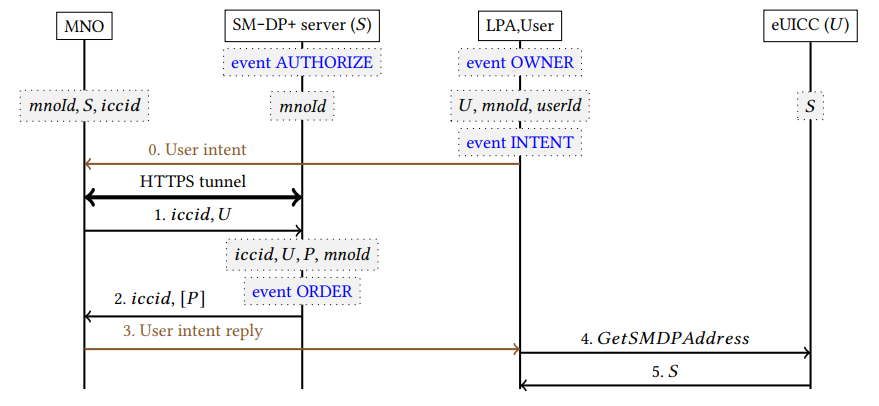
\includegraphics[width=\linewidth]{default-server.png}
\caption{Approccio default server per le fasi di profile ordering e download initialization.}
\label{fig:default-server}
\end{figure}
\begin{figure}
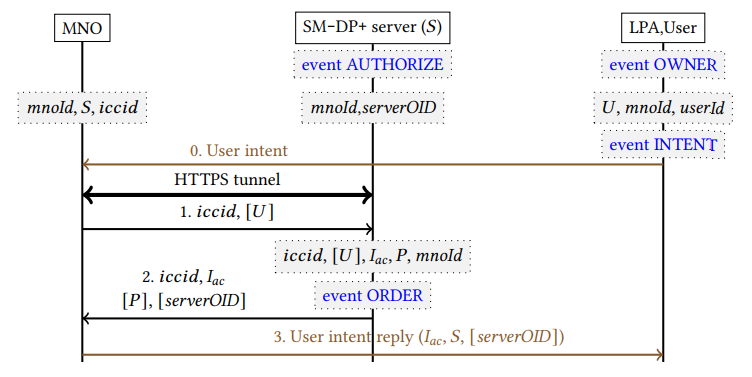
\includegraphics[width=\linewidth]{activation-code.png}
\caption{Approccio activation code per le fasi di profile ordering e download initialization.}
\label{fig:activation-code}
\end{figure}
\begin{figure}
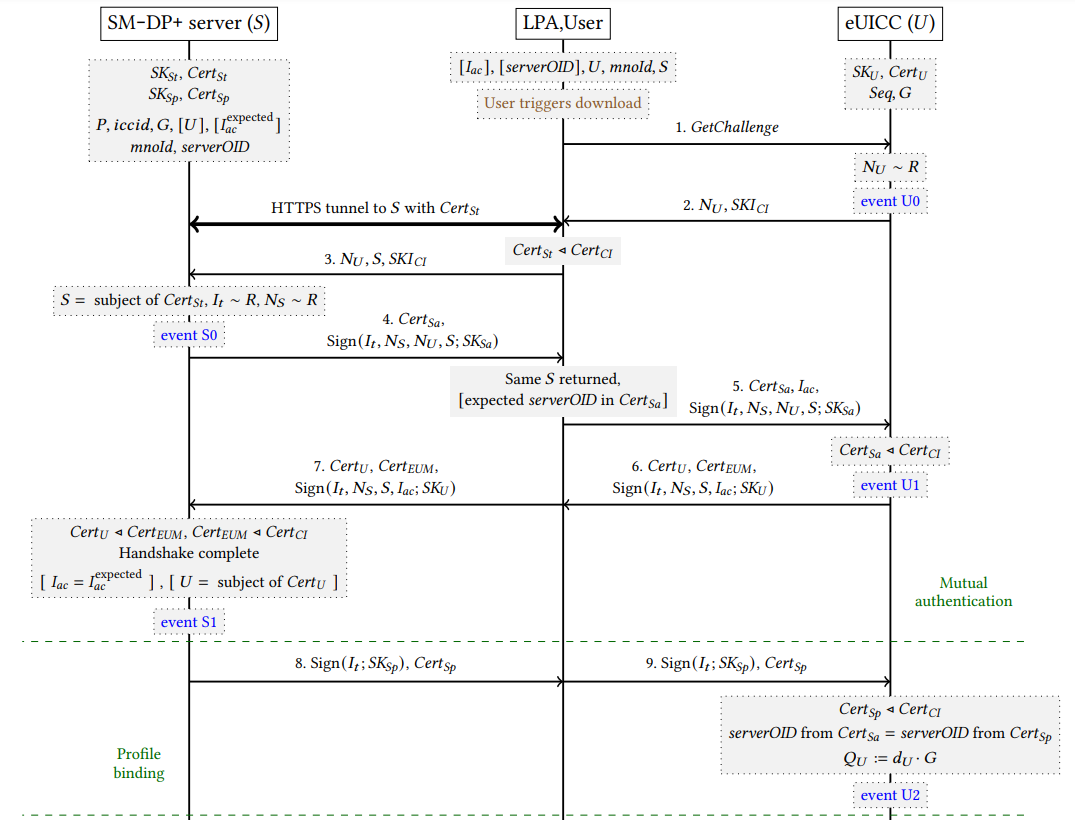
\includegraphics[width=\linewidth]{common-handshake.png}
\caption{Fase di common handshake.}
\label{fig:common-handshake}
\end{figure}
\begin{figure}
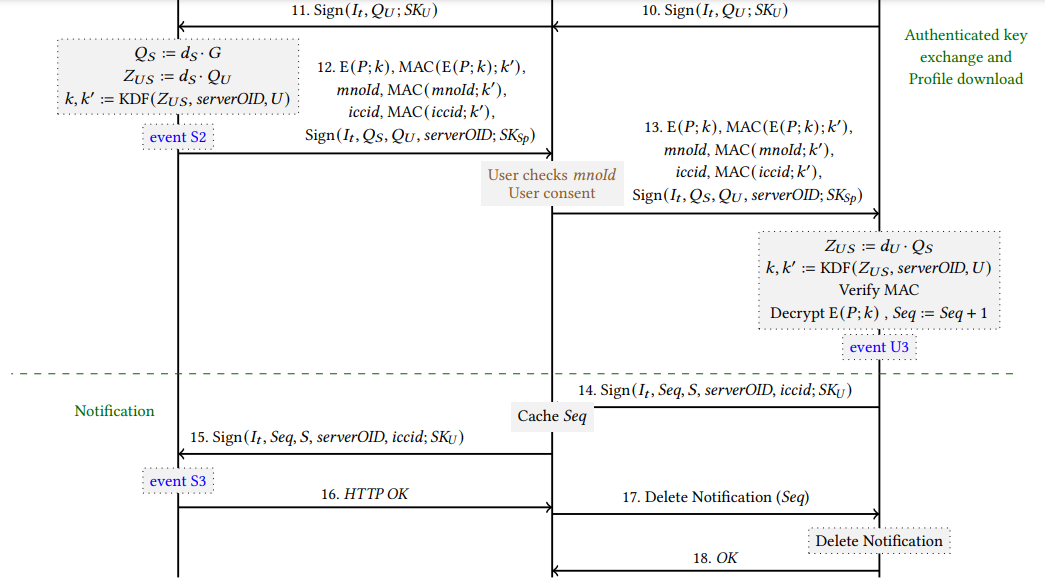
\includegraphics[width=\linewidth]{profile-download.png}
\caption{Fase di profile download.}
\label{fig:profile-download}
\end{figure}

\subsection{Regole per la comunicazione in RSP}
Qualunque comunicazione remota definita per RSP, oltre a prevedere il meccanismo di mutua autenticazione descritto in precedenza, deve far fede alle regole riportate di seguito \cite{GSMA-docs}.
\begin{itemize}
\item \textbf{Privacy dei dati}: l'eUICC, in quanto client, non deve rivelare alcuna informazione privata a un server SM-DP+ non autenticato. Inoltre, non deve generare materiale firmato prima del completamento del processo di autenticazione.
\item \textbf{Protezione della comunicazione}: quando possibile, la comunicazione tra eUICC e server SM-DP+, oltre a essere protetta dall'integrità dei messaggi, dalla cifratura e dall'autenticazione del mittente, dovrebbe essere caratterizzata dalla proprietà di Forward Secrecy. Secondo tale proprietà, se anche una chiave a lungo termine viene compromessa, le chiavi di sessione generate a partire da essa rimangono comunque riservate.
\item \textbf{Autorizzazione}: il server SM-DP+ deve sempre verificare che il client che ha inviato una richiesta sia effettivamente autorizzato prima di far partire l'esecuzione della funzione desiderata.
\end{itemize}

\section{Chiavi crittografiche e certificati}
\subsection{Chiavi crittografiche}
Le chiavi utilizzate dai principali componenti che partecipano all'interazione data dal protocollo RSP sono riportate nella tabella \ref{tab:keys} tratta da \cite{GSMA-docs}.
\begin{table}[h!]
\begin{center}
\captionsetup{skip=4pt}
\caption{Chiavi crittografiche in RSP}
\label{tab:keys}
\begin{tabularx}{\textwidth}{|c|X|}
\hline
\textbf{Nome} & \textbf{Descrizione}\\
\hline
PK.EUICC.ECDSA & Chiave pubblica dell'eUICC usata per verificare le signature dell'eUICC. È inclusa nel certificato CERT.EUICC.ECDSA.\\
\hline
SK.EUICC.ECDSA & Chiave privata dell'eUICC usata per generare le signature. Corrisponde alla chiave $SK_{U}$ citata nella sottosezione \ref{sec:RSP-interaction}.\\
\hline
PK.DPauth.ECDSA & Chiave pubblica del server SM-DP+ usata per verificare le signature del server. È inclusa nel certificato CERT.DPauth.ECDSA.\\
\hline
SK.DPauth.ECDSA & Chiave privata del server SM-DP+ usata per generare le signature per autenticarsi all'eUICC. Corrisponde alla chiave $SK_{Sa}$ citata nella sottosezione \ref{sec:RSP-interaction}.\\
\hline
PK.DPpb.ECDSA & Chiave pubblica del server SM-DP+ usata per verificare le signature del server comprese nel BPP.  È inclusa nel certificato CERT.DPpb.ECDSA.\\
\hline
SK.DPpb.ECDSA & Chiave privata del server SM-DP+ usata per generare le signature per il binding dei profili. Corrisponde alla chiave $SK_{Sp}$ citata nella sottosezione \ref{sec:RSP-interaction}.\\
\hline
PK.DSauth.ECDSA & Chiave pubblica del server SM-DS usata per verificare le signature di SM-DS. È inclusa nel certificato CERT.DSauth.ECDSA.\\
\hline
SK.DSauth.ECDSA & Chiave privata del server SM-DS usata per generare le signature per autenticarsi all'eUICC.\\
\hline
PK.EUM.ECDSA & Chiave pubblica dell'EUM usata per verificare i certificati degli eUICC. È inclusa nel certificato CERT.EUM.ECDSA.\\
\hline
SK.EUM.ECDSA & Chiave privata dell'EUM usata per firmare i certificati degli eUICC.\\
\hline
PK.CI.ECDSA &  Chiave pubblica del CI usata per verificare i certificati dell'EUM dei server SM-DS e del server SM-DP+.\\
\hline
SK.CI.ECDSA & Chiave privata del CI usata per firmare i certificati dell'EUM dei server SM-DS e del server SM-DP+.\\
\hline
otPK.EUICC.ECKA & Chiave pubblica one-time dell'eUICC usata per il key agreement.\\
\hline
otSK.EUICC.ECKA & Chiave privata one-time dell'eUICC usata per il key agreement.\\
\hline
otPK.DP.ECKA & Chiave pubblica one-time del server SM-DP+ usata per il key agreement.\\
\hline
otSK.DP.ECKA & Chiave privata one-time del server SM-DP+ usata per il key agreement.\\
\hline
PK.DP.TLS & Chiave pubblica del server SM-DP+ usata per verificare le signature TLS del server. È inclusa nel certificato CERT.DP.TLS.\\
\hline
SK.DP.TLS & Chiave privata del server SM-DP+ usata per generare le signature per autenticarsi all'LPA. Corrisponde alla chiave $SK_{St}$ citata nella sottosezione \ref{sec:RSP-interaction}.\\
\hline
PK.DS.TLS & Chiave pubblica del server SM-DS usata per verificare le signature TLS di SM-DS. È inclusa nel certificato CERT.DS.TLS.\\
\hline
SK.DS.TLS & Chiave privata del server SM-DS usata per generare le signature per autenticarsi all'LPA.\\
\hline
\end{tabularx}
\end{center}
\end{table}

\subsection{Certificati}
I certificati propri dei principali componenti che partecipano all'interazione data dal protocollo RSP sono riportate nella tabella \ref{tab:cert} tratta da \cite{GSMA-docs}.
\begin{table}[h!]
\begin{center}
\captionsetup{skip=4pt}
\caption{Certificati in RSP}
\label{tab:cert}
\begin{tabularx}{\textwidth}{|c|X|X|}
\hline
\textbf{Nome} & \textbf{Descrizione} & \textbf{Note}\\
\hline
CERT.CI.ECDSA & Certificato GSMA CI & Viene firmato e rilasciato dal CI.\\
\hline
CERT.EUM.ECDSA & Certificato EUM & Viene firmato e rilasciato dal CI. Corrisponde al certificato $Cert_{EUM}$ citato nella sottosezione \ref{sec:RSP-interaction}.\\
\hline
CERT.DPauth.ECDSA & Certificato SM-DP+ per autenticarsi all'eUICC & Viene firmato e rilasciato dal CI. Corrisponde al certificato $Cert_{Sa}$ citato nella sottosezione \ref{sec:RSP-interaction}.\\
\hline
CERT.DPpb.ECDSA & Certificato SM-DP+ per rilasciare e firmare i profili eSIM & Viene firmato e rilasciato dal CI. Corrisponde al certificato $Cert_{Sp}$ citato nella sottosezione \ref{sec:RSP-interaction}.\\
\hline
CERT.DP.TLS & Certificato TLS di SM-DP+ & Viene firmato e rilasciato dal CI. Corrisponde al certificato $Cert_{St}$ citato nella sottosezione \ref{sec:RSP-interaction}.\\
\hline
CERT.DSauth.ECDSA & Certificato SM-DS & Viene firmato e rilasciato dal CI.\\
\hline
CERT.DS.TLS & Certificato TLS di SM-DS & Viene firmato e rilasciato dal CI.\\
\hline
CERT.EUICC.ECDSA & Certificato eUICC & Viene firmato e rilasciato dall'EUM.\\
\hline
\end{tabularx}
\end{center}
\end{table}
\\La figura \ref{fig:cert-chain} tratta da \cite{GSMA-docs} definisce uno schema riassuntivo della catena di certificati definita dalla Public Key Infrastructure (PKI) di RSP.
\begin{figure}
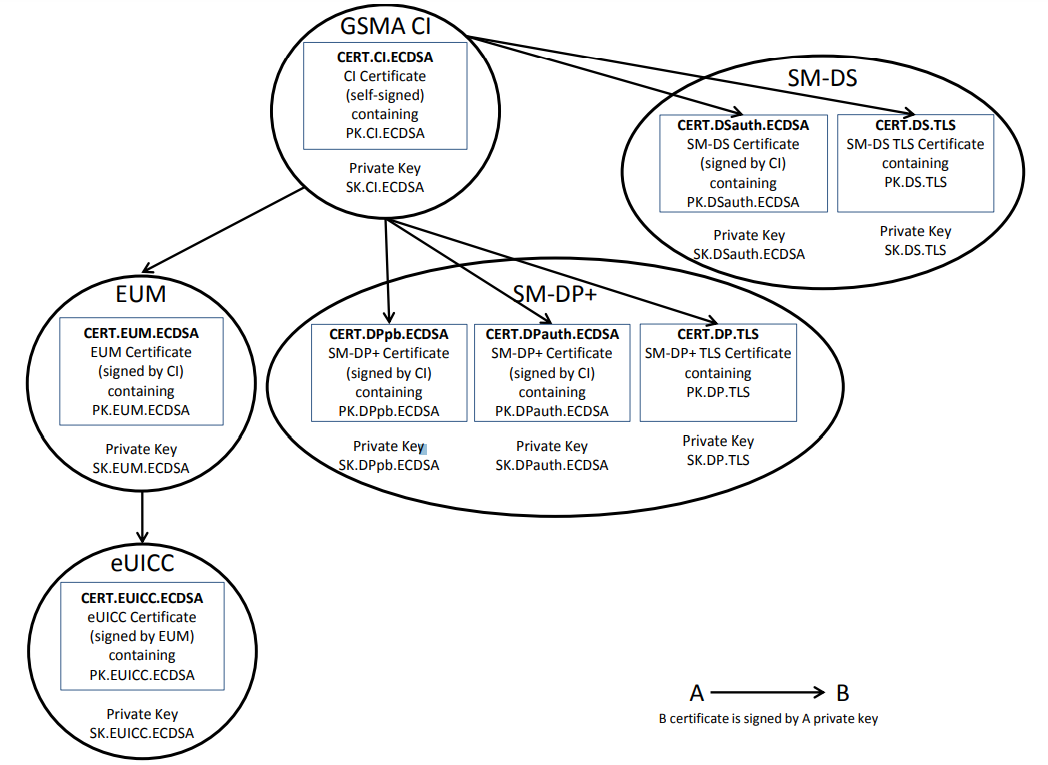
\includegraphics[width=\linewidth]{cert-chain.png}
\caption{Catena di certificati definita dalla PKI di RSP.}
\label{fig:cert-chain}
\end{figure}
All'interno della PKI, il Certificate Issuer di GSMA (CI) è la Root Certification Authority del servizio RSP e, di conseguenza, rappresenta il nodo radice della catena. La figura \ref{fig:cert-chain}, inoltre, rimarca bene come tutti i certificati siano rilasciati dal CI, fatta eccezione di CERT.EUICC.ECDSA che, invece, viene rilasciato dall'EUM. Tutti i certificati rilasciati direttamente dal CI possono essere revocati in qualunque momento, in particolar modo se le entità corrispondenti (CI, EUM, SM-DP+, SM-DS) vengono compromesse. D'altra parte, i certificati eUICC (CERT.EUICC.ECDSA) non vengono revocati in modo individuale: di fatto, è difficile che un singolo eUICC venga compromesso. Piuttosto, è più verosimile che un modello eUICC o un intero batch di produzione di eUICC venga dichiarato come compromesso; quando ciò avviene, quello che si fa è revocare direttamente il certificato EUM (CERT.EUM.ECDSA) associato a quel modello o batch di produzione di eUICC \cite{GSMA-docs}.\\
Il CI fornisce una Certificate Revocation List (CRL), che è la lista dei certificati revocati tra tutti i certificati non scaduti che erano stati rilasciati da quello stesso CI. Ciascun CI, per giunta, deve pubblicare la propria CRL sia periodicamente, sia ogni volta che viene revocato un particolare certificato \cite{GSMA-docs}.\\
In realtà, i certificati relativi alla PKI di RSP di cui si è discusso finora non sono gli unici certificati utilizzati per effettuare il deployment dei profili eSIM: esiste anche un certificato per firmare l'applicazione LPA e un certificato da inserire in ciascun profilo eSIM da distribuire all'end user. Dove entrano in gioco tali certificati? Con riferimento alla guida di Android per le API e per l'implementazione del deployment dei profili eSIM \cite{Android-docs}, l'interazione tra un'applicazione LPA e l'interfaccia all'eUICC (legata al componente EuiccManager in \cite{Android-docs}) può avvenire solo se l'applicazione dispone dei privilegi dell'operatore. Di norma, tali privilegi sono conferiti all'applicazione se il certificato usato per firmarla coincide col certificato presente nel profilo fornito da SM-DP+.

\section{Ciclo di vita dei profili in SM-DP+}
La tabella \ref{tab:profile-states} tratta da \cite{GSMA-docs} fornisce un elenco degli stati in cui ciascun profilo eSIM può trovarsi nell'arco della sua esistenza.
\begin{table}[h!]
\begin{center}
\captionsetup{skip=4pt}
\caption{Stati dei profili eSIM}
\label{tab:profile-states}
\begin{tabularx}{\textwidth}{|c|X|}
\hline
\textbf{Nome} & \textbf{Descrizione}\\
\hline
Available & Il profilo è disponibile nell’inventory del server SM-DP+.\\
\hline
Allocated & Il profilo è riservato per il download senza essere linkato a un EID (eUICC ID).\\
\hline
Linked & Il profilo è riservato per il download ed è linkato a un EID.\\
\hline
Confirmed & Il profilo è riservato per il download (che sia esso linkato o non linkato a un EID) col matching ID (i.e. il codice che identifica la transazione di download) e il codice di conferma (i.e. il codice che deve essere inserito dall'end user), se richiesti.\\
\hline
Released & Il profilo è pronto per il download e l’installazione dopo che l’operatore ha effettuato la configurazione di rete.\\
\hline
Downloaded & Il profilo è stato consegnato all’LPA (i.e. è stato scaricato).\\
\hline
Installed & Il profilo è stato installato sull’eUICC con successo.\\
\hline
Error & Il profilo non è stato installato a causa di una condizione di errore.\\
\hline
Unavailable & Il profilo non può essere più riutilizzato da SM-DP+.\\
\hline
\end{tabularx}
\end{center}
\end{table}
\\Nelle figure \ref{fig:profile-states1}, \ref{fig:profile-states2} tratte da \cite{GSMA-docs} sono mostrati due diagrammi a stati finiti che illustrano per bene il ciclo di vita dei profili in SM-DP+.
\begin{figure}
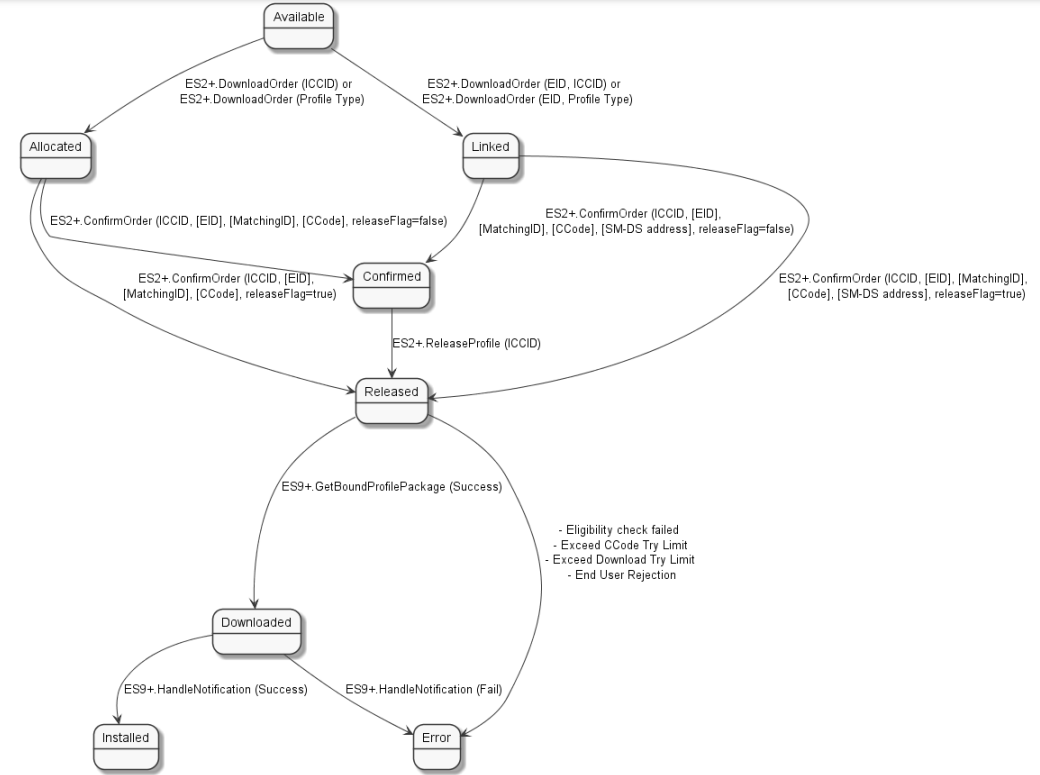
\includegraphics[width=\linewidth]{profile-states1}
\caption{Primo diagramma a stati per i profili eSIM.}
\label{fig:profile-states1}
\end{figure}
\begin{figure}
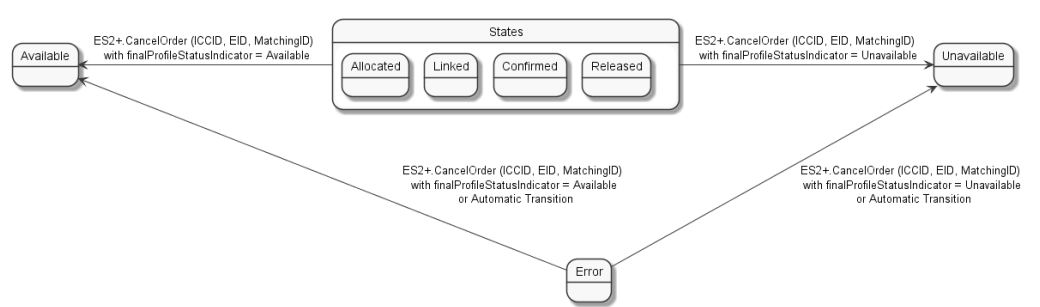
\includegraphics[width=\linewidth]{profile-states2}
\caption{Secondo diagramma a stati per i profili eSIM.}
\label{fig:profile-states2}
\end{figure}
\\Con riferimento alla figura \ref{fig:profile-states1}, a partire dallo stato Available:
\begin{itemize}
\item Si passa allo stato Allocated se si effettua l'ordine di download senza specificare l'EID.
\item Si passa allo stato Linked se si effettua l'ordine di download specificando l'EID.
\end{itemize}
A partire dallo stato Allocated:
\begin{itemize}
\item Si passa allo stato Confirmed se si conferma l'ordine di download con releaseFlag=false.
\item Si passa allo stato Released se si conferma l'ordine di download con releaseFlag=true.
\end{itemize}
A partire dallo stato Linked:
\begin{itemize}
\item Si passa allo stato Confirmed se si conferma l'ordine di download con releaseFlag=false.
\item Si passa allo stato Released se si conferma l'ordine di download con releaseFlag=true.
\end{itemize}
A partire dallo stato Confirmed:
\begin{itemize}
\item Si passa allo stato Released se si effettua il rilascio del profilo in modo tale che sia effettivamente pronto per il download e l'installazione.
\end{itemize}
A partire dallo stato Released:
\begin{itemize}
\item Si passa allo stato Downloaded se il profilo viene consegnato all'LPA con successo.
\item Si passa allo stato Error se si ha un errore nel consegnare il profilo all'LPA.
\end{itemize}
A partire dallo stato Downloaded:
\begin{itemize}
\item Si passa allo stato Installed se il profilo viene installato sull'eUICC con successo.
\item Si passa allo stato Error se si ha un errore nell'installare il profilo sull'eUICC.
\end{itemize}
Con riferimento alla figura \ref{fig:profile-states2}, a partire dagli stati Allocated / Linked / Confirmed / Released:
\begin{itemize}
\item Si torna allo stato Available se l'ordine di download viene annullato con finalProfileStatusIndicator=Available.
\item Si passa allo stato Unavailable se l'ordine di download viene annullato con finalProfileStatusIndicator=Unavailable.
\end{itemize}
A partire dallo stato Error:
\begin{itemize}
\item Si torna allo stato Available in modo automatico oppure se l'ordine di download viene annullato con finalProfileStatusIndicator=Available.
\item Si passa allo stato Unavailable in modo automatico oppure se l'ordine di download viene annullato con finalProfileStatusIndicator=Unavailable.
\end{itemize}

\chapter{Sicurezza dell'eSIM a run-time}
[TODO]

\chapter{Sicurezza dell'eSIM a boot-time}
\section{Funzionamento del boot dell'eSIM}
[TODO]

\section{Potenziali vulnerabilità}
[TODO]

\section{Prove sperimentali}
[TODO]

\chapter{Conclusione}
[TODO]

\bibliography{Bibliography}

\chapter*{Ringraziamenti}
[TODO]

\end{document}